After going through all the unscrambling of the system. You are now be able to listen to the scrambled noise. Which for our group is played.

From there to here from here to there funny things are everywhere

\begin{figure}[!htbp]
  \centering
    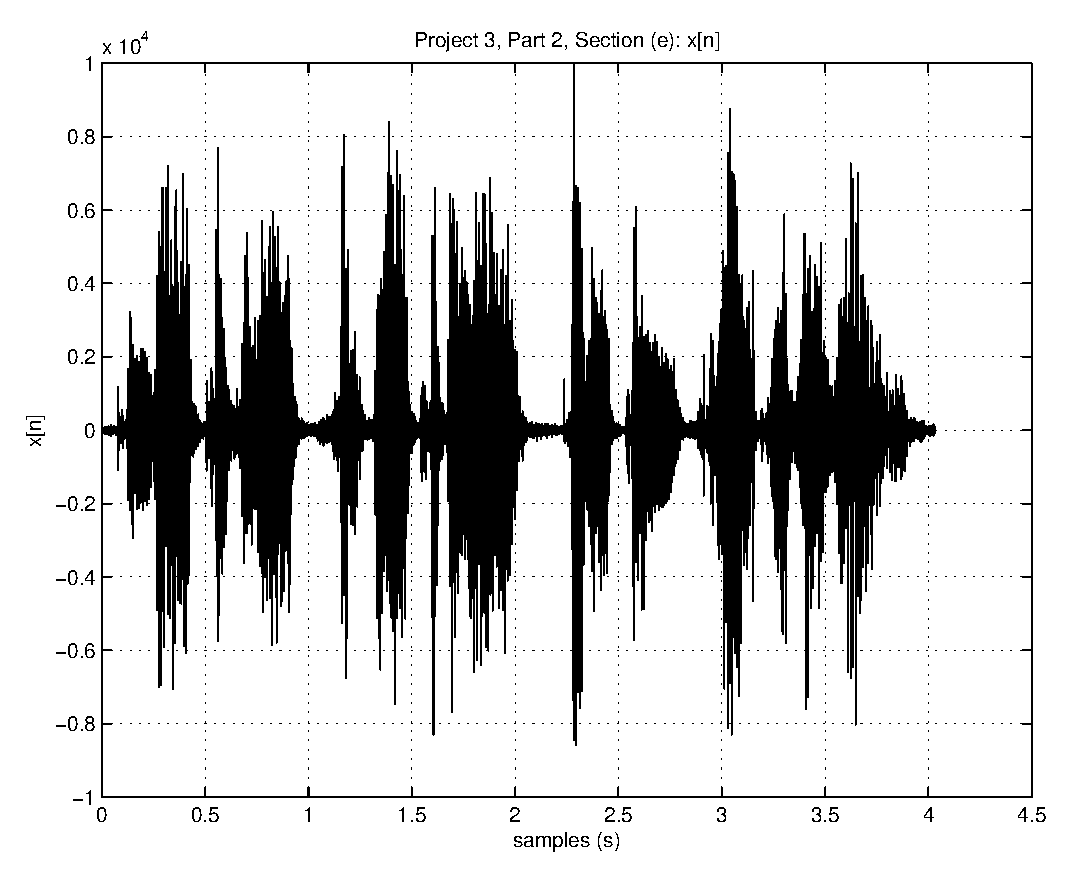
\includegraphics[width=0.7\textwidth]{Part2/Output/Figures/Part2E-1.eps}
  \caption{Output For E in Part 2}
\end{figure}

\begin{figure}[!htbp]
  \centering
    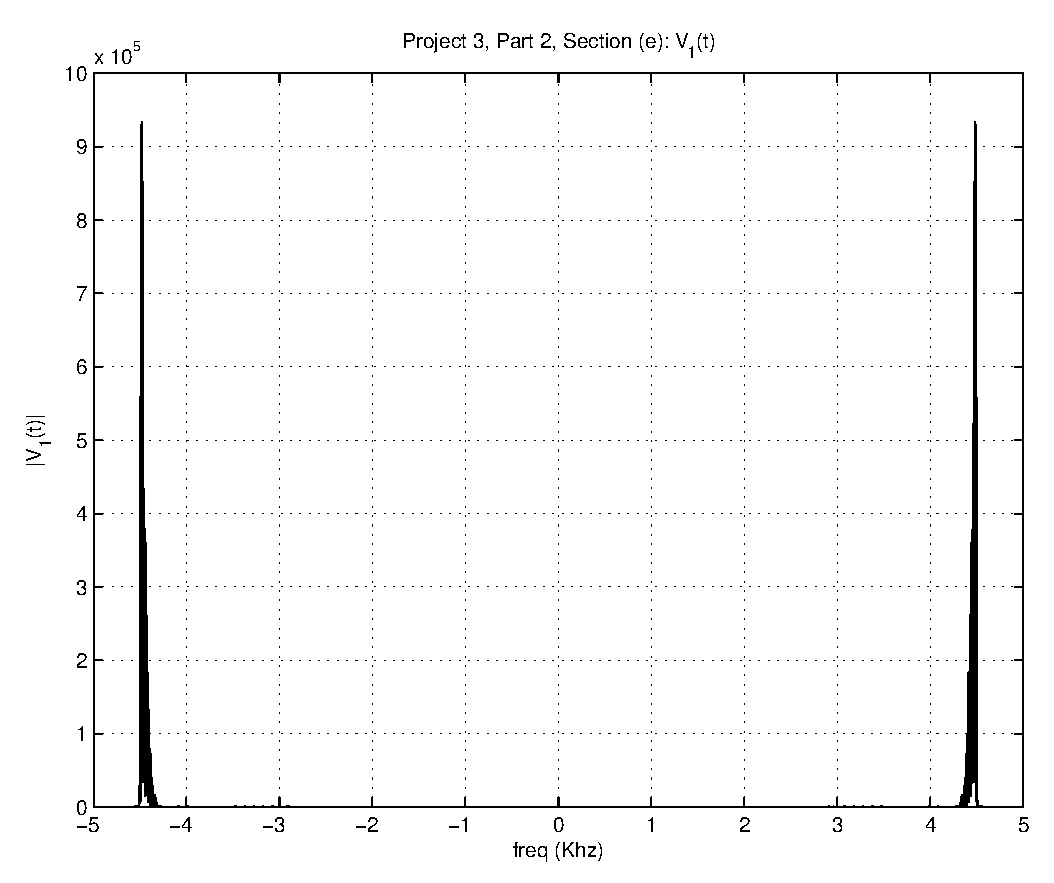
\includegraphics[width=0.7\textwidth]{Part2/Output/Figures/Part2E-2.eps}
  \caption{Output For E in Part 2}
\end{figure}

\begin{figure}[!htbp]
  \centering
    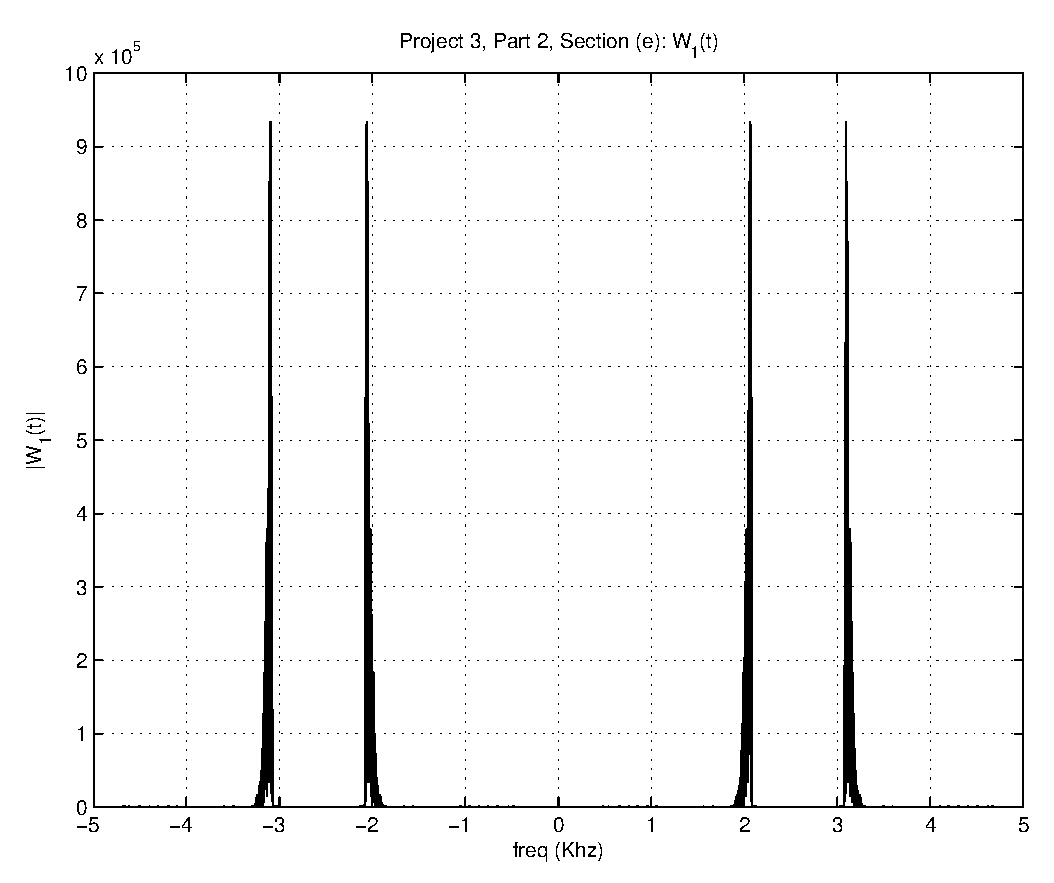
\includegraphics[width=0.7\textwidth]{Part2/Output/Figures/Part2E-3.eps}
  \caption{Output For E in Part 2}
\end{figure}

\begin{figure}[!htbp]
  \centering
    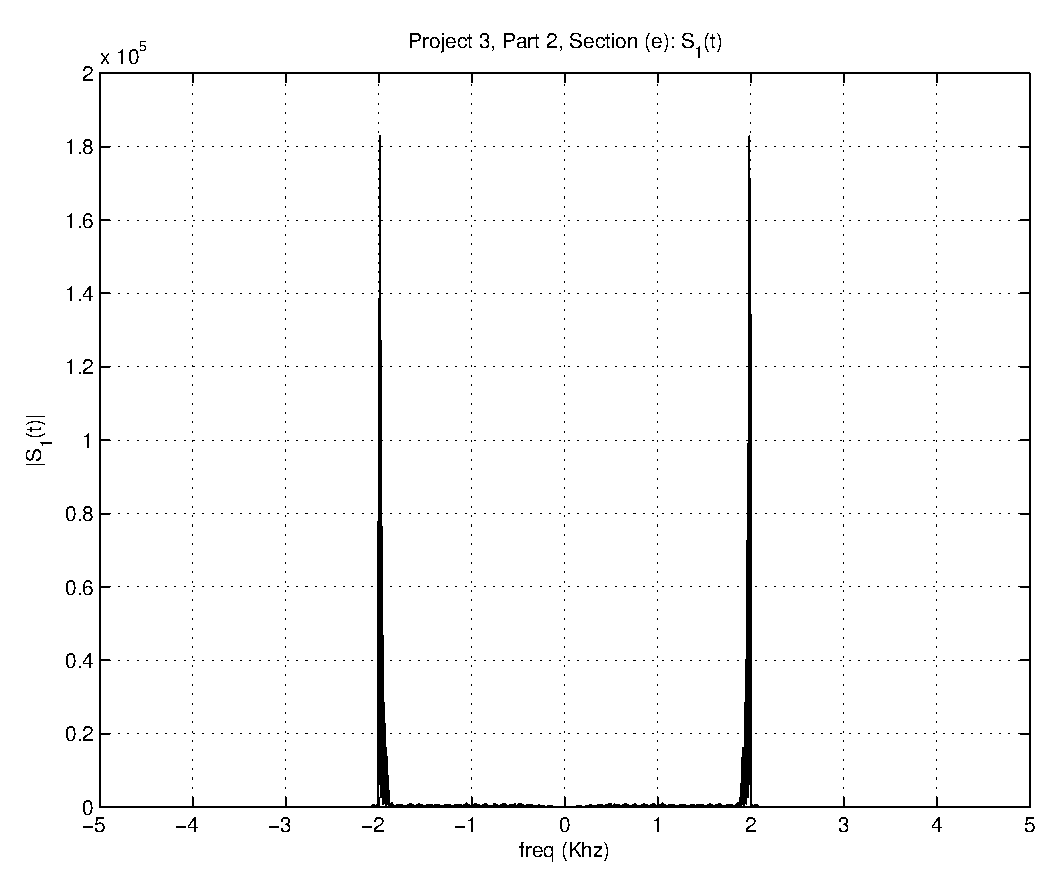
\includegraphics[width=0.7\textwidth]{Part2/Output/Figures/Part2E-4.eps}
  \caption{Output For E in Part 2}
\end{figure}

\begin{figure}[!htbp]
  \centering
    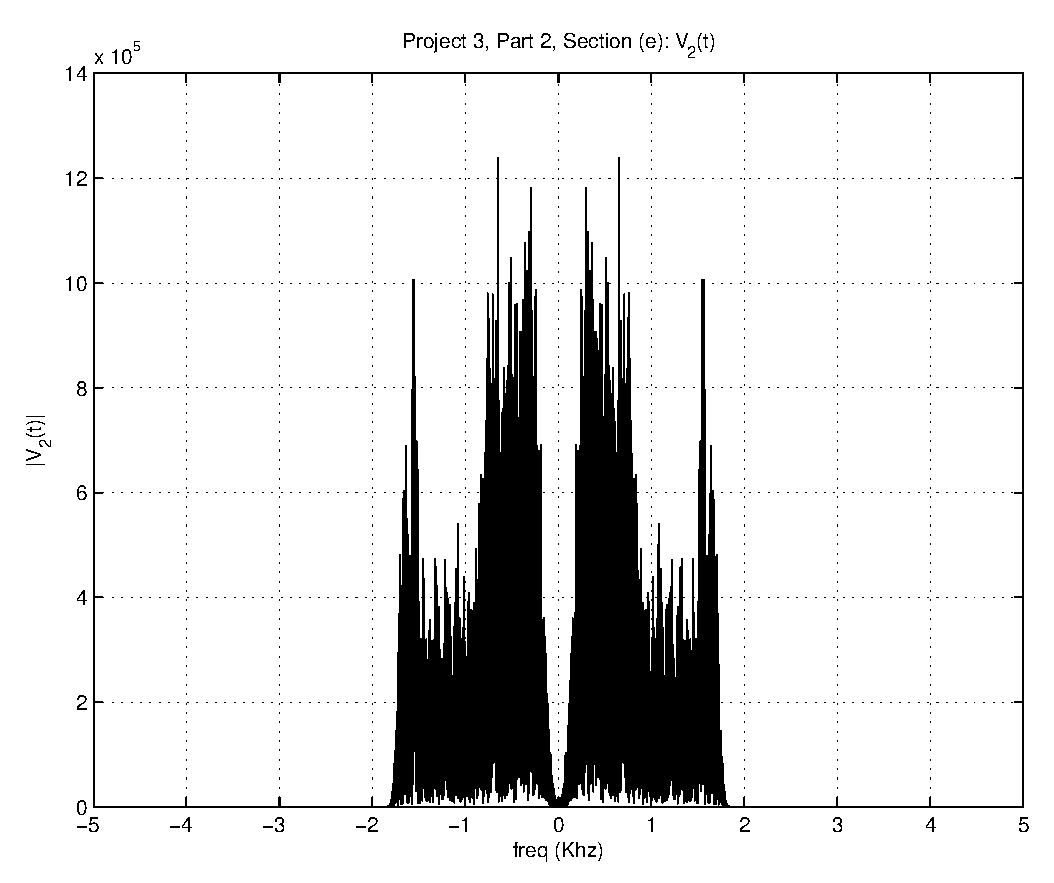
\includegraphics[width=0.7\textwidth]{Part2/Output/Figures/Part2E-5.eps}
  \caption{Output For E in Part 2}
\end{figure}

\begin{figure}[!htbp]
  \centering
    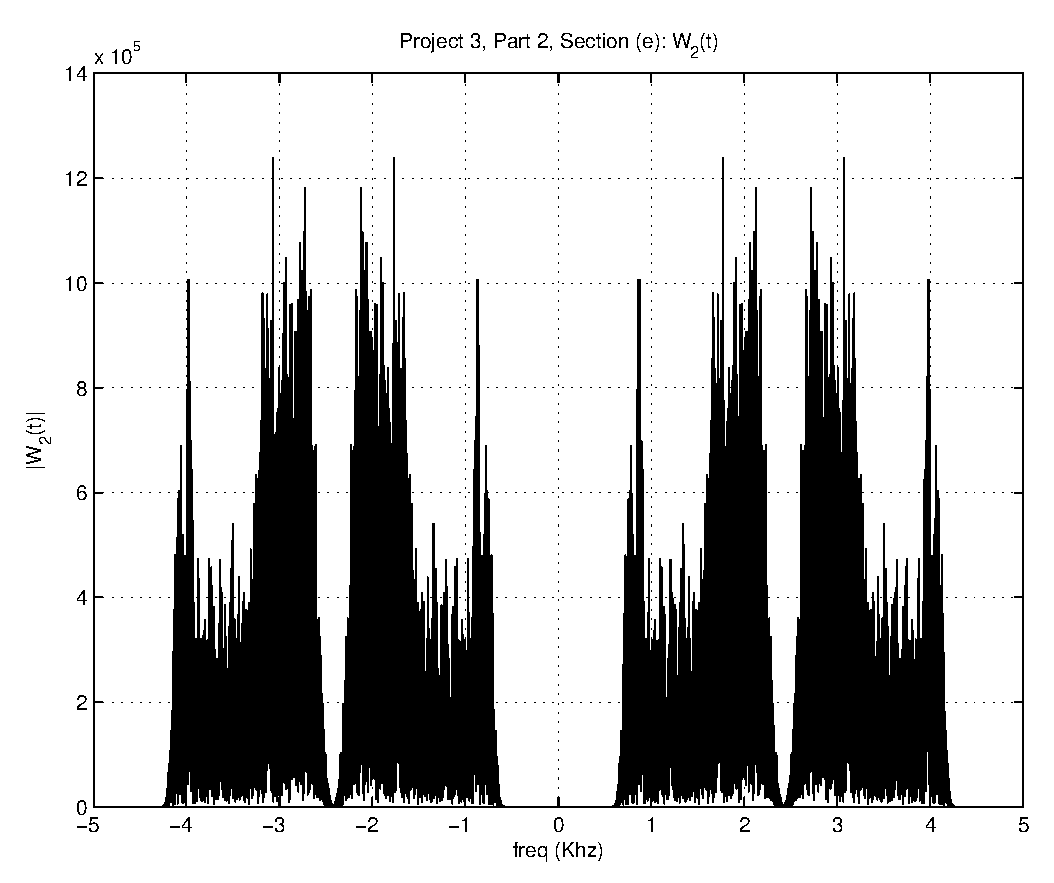
\includegraphics[width=0.7\textwidth]{Part2/Output/Figures/Part2E-6.eps}
  \caption{Output For E in Part 2}
\end{figure}

\begin{figure}[!htbp]
  \centering
    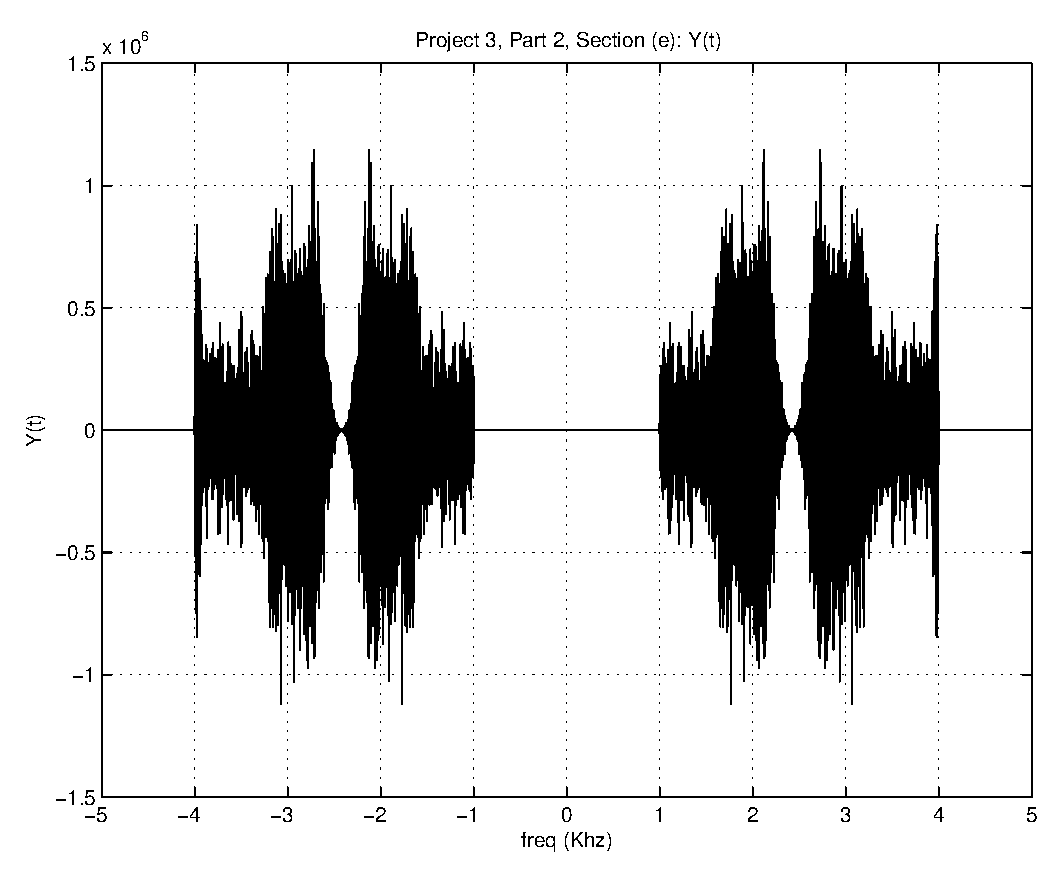
\includegraphics[width=0.7\textwidth]{Part2/Output/Figures/Part2E-7.eps}
  \caption{Output For E in Part 2}
\end{figure}

